\documentclass[12pt,a4paper]{article}
\usepackage{tikz}
\usetikzlibrary{arrows.meta,positioning}
\usepackage{tabularx}
\usepackage{graphicx}
\usepackage{amsmath}
\usepackage{amssymb}
\usepackage{amsthm}
\usepackage{bm}
\usepackage{hyperref}
\usepackage{booktabs}
\usepackage{array}
\usepackage{geometry}
\geometry{margin=2.5cm}
\hypersetup{colorlinks=true, linkcolor=blue, citecolor=blue, urlcolor=blue}
\newtheorem{theorem}{Theorem}
\newtheorem{proposition}{Proposition}
\newtheorem{definition}{Definition}
\newtheorem{lemma}{Lemma}
\newtheorem{corollary}{Corollary}
\newtheorem{criterion}{Criterion}




\title{\textbf{Paper B-05: Neural Computation:\\ A Constraint-Driven Flux Dynamics (CDFD) Perspective}}
\author{Steve Bico Mujjabi, MD\\
\small Independent Researcher\\
\small Founder, Vura Labs\\
\small Kampala, Uganda\\
\small ORCID: 0009-0001-0556-5516}
\date{May 2026}


\newcommand{\EarthSuppPath}{Part\_A\_Earth\_Systems/supplementary/supplementary\_earth\_}
\newcommand{\EngSuppPath}{Part\_B\_Engineered\_Systems/supplementary/supplementary\_eng\_}
\newcommand{\SocSuppPath}{Part\_C\_Socioeconomic\_Systems/supplementary/supplementary\_soc\_}
\newcommand{\DomainSuppPath}{Part\_D\_Domain\_Applications/supplementary/supplementary\_dom\_}
\begin{document}
\maketitle

\begin{abstract}
This paper treats neural computation as an engineered and biological transport
analogy for CDFD/AFL. Spikes, synaptic current, activation flow, gradients, and
attention-like routing are read as candidate fluxes $\Phi$ moving through
constraints $C$ such as bandwidth, inhibition, metabolic cost, finite precision,
and connectivity. The paper does not claim that biological brains and artificial
networks are the same material system. It asks which measurable bottlenecks and
memory terms make neural computation auditable.
\end{abstract}

\section*{Symbol Conventions}

\noindent\textbf{CDFD/AFL Part IV symbol convention.}
\begin{center}
{\small
\begin{tabular}{p{0.15\linewidth}p{0.34\linewidth}p{0.41\linewidth}}
\hline
Symbol & Part IV meaning & Cross-domain reading \\
\hline
$\Phi$ & Driving flux or throughput & Energy, matter, signal, capital, information, traffic, force, or biological load entering a system \\
$C$ & Active constraint or capacity burden & Bottleneck, resistance, boundary, scarcity, toxicity, regulation, topology, latency, or load-bearing limit \\
$S$ & Responsiveness or adaptive surface & The system's ability to reconfigure, buffer, route, repair, learn, or preserve function under changing load \\
$M_s$ & Structural memory & Stored damage, hysteresis, inherited topology, institutional memory, trained weights, ecological legacy, or retained state \\
$\Psi_s$ & Adaptive operating ratio $(\Phi/C)\cdot S\cdot M_s$ & Local bookkeeping gauge for constrained operation, overload, recovery, or regime change; not a universal constant \\
$\Lambda$ & Life Number or capstone surplus ratio where explicitly defined & Reserved for Part II-derived life-number notation or synthesis-level surplus measures, never an undefined decoration \\
\hline
\end{tabular}
}
\end{center}

\noindent\textbf{Greek-symbol convention.}
\begin{center}
{\small
\begin{tabular}{p{0.15\linewidth}p{0.34\linewidth}p{0.41\linewidth}}
\hline
Symbol & Local role & Interpretation rule \\
\hline
$\alpha$ & Accumulation or reinforcement coefficient & Sets how fast a pathway, constraint, habit, cascade, or retained structure grows under load \\
$\beta$ & Relaxation, decay, clearance, or washout coefficient & Sets loss, recovery, damping, forgetting, degradation, or return toward baseline \\
$\gamma$ & Coupling, diffusion, redistribution, or transfer coefficient & Sets spread across nodes, layers, tissues, markets, infrastructures, media, or physical phases \\
$\delta,\epsilon$ & Perturbation, tolerance, small offset, or numerical guard & Used only as local thresholds, stability margins, measurement tolerances, or stress increments \\
$\eta,\lambda,\mu,\nu$ & Efficiency, rate, baseline, intensity, or frequency terms & Meaning is fixed by the equation, subscript, and domain-specific proxy in the paragraph where the term appears \\
$\rho,\sigma,\tau,\phi$ & Density/correlation, variability/noise, time-scale, phase, or field terms & Local coefficients only; subscripts bind them to the named pathway, domain, or experiment \\
$\Omega,\Lambda$ & Domain/state space; Life Number where defined & $\Omega$ names a modeled state space; $\Lambda$ carries life-number or synthesis notation only when the paper defines it \\
\hline
\end{tabular}
}
\end{center}

\section{Series Context}

Part I sets the flow--constraint language used here \cite{MujjabiPartI2026}.
Part II develops the Life Number and the origins-of-life use of the same notation
\cite{MujjabiPartII2026}. Part III applies AFL to biology and medicine
\cite{MujjabiPartIII2026}. Part IV \cite{MujjabiPartIV2026}, DOI \url{https://doi.org/10.5281/zenodo.20395901}, supplies the
cross-domain stress-test archive. This paper sits in Part B because it focuses
on the engineered-computation reading of neural systems.

\section{Neural Computation as Transport}

Neural computation moves signals through constrained pathways. In biological
tissue, those constraints include synaptic strength, inhibition, refractory
periods, metabolic cost, and network topology. In artificial neural networks,
they include parameter count, activation bandwidth, context length, memory
traffic, precision, optimization state, and hardware limits. CDFD/AFL gives a
single audit question for both settings: where does flow concentrate, what
limits it, how does the system adapt, and what past load remains in the
structure?

\section{Candidate Variable Map}

\begin{table}[h]
\centering
\begin{tabularx}{\textwidth}{@{}lXX@{}}
\toprule
CDFD term & Neural-computation reading & Example proxy \\
\midrule
$\Phi$ & signal, activation, or gradient flow & spike rate, activation norm, token updates \\
$C$ & active constraint & inhibition, bandwidth, precision, memory traffic \\
$S$ & responsiveness & plasticity, gating, normalization, routing adjustment \\
$M_s$ & structural memory & synaptic weights, trained parameters, cached state \\
$\Psi_s$ & operating ratio & balanced, saturated, unstable, or underused regime \\
\bottomrule
\end{tabularx}
\end{table}

\section{Biological and Engineered Boundaries}

Part III gives the biological and medical context for AFL \cite{MujjabiPartIII2026}.
This paper uses that context carefully. A biological neuron, a neuromorphic
device, and a transformer layer can all be described as constrained signal
systems, but the measurements differ. A useful comparison must state the unit
of flow, the time scale, the constraint, and the failure mode before drawing
any cross-domain conclusion.

\section{Measurement Layer}

For biological data, measurable proxies may include firing rate, synaptic
current, local field power, metabolic demand, refractory recovery, and plastic
change. For artificial systems, proxies may include activation magnitude,
gradient norm, attention entropy, memory bandwidth, context pressure, and
inference latency. CDFD/AFL adds value only if these proxies improve the audit
of saturation, collapse, recovery, or adaptation.

\section{Current Runtime Diagnostic}

The Part B adapter sweep includes artificial-intelligence and computation rows,
and the Part E cascade test records finite runtime behavior in the current CDFD
Runtime \cite{CDFDRuntime2026}. These files document model behavior. They do
not validate a neuroscience claim or certify an AI-system claim.

\section{Tests That Can Break the Mapping}

The mapping weakens if measured bottlenecks do not track saturation or recovery,
if ordinary neural-network or neuroscience metrics explain the behavior more
cleanly, or if the proposed variables cannot be measured without circular
definitions.

% BEGIN PART IV MAJOR UNIVERSAL UPGRADE
\section{Major Universal Upgrade: Mechanism, Scale, and Tests}

\subsection{Observable Translation}

The paper-specific translation begins with an observable chain rather than a
verbal analogy. For Neural Computation, the proposed drive is signals, training examples, gradients, and inference demand.
The active limitation is compute, data quality, architecture, bandwidth, and noise. Responsiveness is carried by
learning, attention, sparsity, regularization, and plasticity, while retained state is represented by
weights, optimizer state, replay history, and accumulated bias. The outcome to explain is accuracy, calibration, generalization, and adaptation.

\begin{table}[htbp]
\centering
\small
\caption{Operational CDFD/AFL map for Paper B-05.}
\begin{tabularx}{\textwidth}{|l|X|X|}
\hline
\textbf{Term} & \textbf{Paper-specific observable meaning} & \textbf{Measurement question} \\
\hline
$\Phi$ & signals, training examples, gradients, and inference demand & What rate, load, gradient, or demand enters the focal system? \\
\hline
$C$ & compute, data quality, architecture, bandwidth, and noise & Which measured bottleneck limits transfer, function, or recovery? \\
\hline
$S$ & learning, attention, sparsity, regularization, and plasticity & Which process changes effective capacity or reroutes the load? \\
\hline
$M_s$ & weights, optimizer state, replay history, and accumulated bias & Which retained state makes equal present loads produce different futures? \\
\hline
$Y$ & accuracy, calibration, generalization, and adaptation & Which outcome is predicted out of sample, with uncertainty? \\
\hline
\end{tabularx}
\end{table}

\begin{figure}[htbp]
\centering
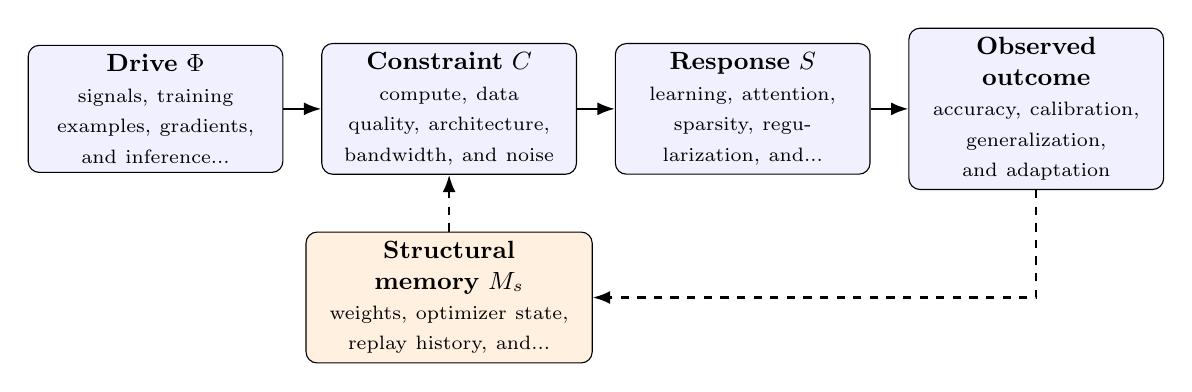
\begin{tikzpicture}[
    node distance=0.48cm,
    every node/.style={font=\small},
    box/.style={draw, rounded corners, align=center, minimum height=1.45cm, text width=3.0cm, fill=blue!6},
    memory/.style={draw, rounded corners, align=center, minimum height=1.25cm, text width=3.4cm, fill=orange!12},
    flow/.style={-{Latex[length=2.2mm]}, thick},
    feedback/.style={-{Latex[length=2.2mm]}, thick, dashed}
]
\node[box] (drive) {\textbf{Drive $\Phi$}\\\scriptsize signals, training examples, gradients, and inference...};
\node[box, right=of drive] (constraint) {\textbf{Constraint $C$}\\\scriptsize compute, data quality, architecture, bandwidth, and noise};
\node[box, right=of constraint] (response) {\textbf{Response $S$}\\\scriptsize learning, attention, sparsity, regularization, and...};
\node[box, right=of response] (outcome) {\textbf{Observed outcome}\\\scriptsize accuracy, calibration, generalization, and adaptation};
\node[memory, below=0.72cm of constraint] (memory) {\textbf{Structural memory $M_s$}\\\scriptsize weights, optimizer state, replay history, and...};
\draw[flow] (drive) -- (constraint);
\draw[flow] (constraint) -- (response);
\draw[flow] (response) -- (outcome);
\draw[feedback] (outcome.south) |- (memory.east);
\draw[feedback] (memory.north) -- (constraint.south);
\end{tikzpicture}
\caption{Paper B-05 observable CDFD/AFL architecture for Neural Computation. Solid arrows give the proposed forward chain; dashed arrows make history-dependent feedback explicit.}
\label{fig:b05-architecture}
\end{figure}

\subsection{Minimal Coupled Model}

A paper-level model must separate throughput, constraint accumulation, response,
and history. One deliberately minimal form is
\begin{align}
Y(t) &= \frac{\Phi(t)S(t)}{\epsilon + C(t)}, \\
\frac{dC}{dt} &= \alpha \Phi(t) - \beta S(t)C(t) + \gamma \mathcal{L}C(t), \\
\frac{dM_s}{dt} &= \eta C(t) - \mu M_s(t), \\
\Psi_s(t) &= \frac{\widehat{\Phi}(t)}{\epsilon+\widehat{C}(t)}\,
             \widehat{S}(t)\,[1+\omega\widehat{M_s}(t)] .
\end{align}
Here $Y$ is the measured output, $\epsilon>0$ prevents a singular denominator,
$\mathcal{L}$ is a spatial or network coupling operator, and hats denote
explicitly normalized variables. The sign and magnitude of $\omega$ must be
estimated: memory can preserve useful organization or amplify damage. No fixed
threshold is universal before the variables, normalization, and observation
scale are declared.

For this paper, the hypothesized causal sequence is specific. A change in
signals, training examples, gradients, and inference demand arrives faster than learning, attention, sparsity, regularization, and plasticity can compensate.
This raises or redistributes compute, data quality, architecture, bandwidth, and noise. If the load persists,
the retained state encoded by weights, optimizer state, replay history, and accumulated bias changes the next response, so a later event of equal
magnitude can produce a different trajectory in accuracy, calibration, generalization, and adaptation. The
scientific task is to estimate that sequence against the best ordinary model of
the domain, not merely to redescribe the outcome after it occurs.

\subsection{Cross-Scale Universality Without Mechanistic Erasure}

For the engineered systems family, the universal comparison is between demand, designed capacity, feedback control, dependency topology, and accumulated technical state. The strongest engineering use is prospective: the mapping must identify a bottleneck, a control action, or a recovery signature before the failure occurs. \cite{BarabasiAlbert1999,WattsStrogatz1998,Shannon1948,BakTangWiesenfeld1987}
The CDFD programme is cumulative: Part I supplies the flow--constraint
foundation \cite{MujjabiPartI2026}; Part II asks when maintained throughput
supports persistent organized states \cite{MujjabiPartII2026}; Part III
develops adaptive limitation and biological memory \cite{MujjabiPartIII2026};
and Part IV \cite{MujjabiPartIV2026} tests how much of that architecture
survives translation. The CDFD Runtime \cite{CDFDRuntime2026} supplies a
reproducible numerical stress surface, but it does not substitute for the
domain evidence named here.

The required scale declaration for this paper is nanoseconds to model lifetimes; units to learning ecosystems. At short
scales, the key question is whether the incoming drive is transmitted,
buffered, or diverted. At intermediate scales, response changes effective
capacity and network exposure. At long scales, retained structure can alter the
state space itself. A result is genuinely cross-scale only when the aggregation
rule is stated and the same conclusion is not an artifact of averaging.

\subsection{Evidence Ladder and Discriminating Tests}

\begin{table}[htbp]
\centering
\small
\caption{Evidence ladder for Paper B-05. Each rung can fail independently.}
\begin{tabularx}{\textwidth}{|p{0.17\textwidth}|X|X|}
\hline
\textbf{Test} & \textbf{Design} & \textbf{Discriminating result} \\
\hline
Proxy audit & Measure learning curves, activation traces, gradient statistics, ablations, and benchmark shifts and preregister how each record maps to $\Phi$, $C$, $S$, $M_s$, and $Y$. & The mapping fails if proxies are non-identifiable, circular, or change meaning across cases. \\
\hline
Load ramp & Apply or observe a distribution shift or capacity bottleneck after training while estimating the dominant constraint and response time. & A threshold claim requires a reproducible nonlinear change and uncertainty bounds, not a visually chosen breakpoint. \\
\hline
Recovery and memory & Match present load across units with different histories, then compare recovery paths. & The memory claim requires history-dependent divergence after current conditions are controlled. \\
\hline
Model comparison & Compare the baseline domain model with and without the CDFD/AFL state variables using held-out data. & The paper's stated falsifier is: explicit constraint-memory variables do not improve generalization or adaptation forecasts. \\
\hline
\end{tabularx}
\end{table}

The strongest practical design combines a prospective perturbation with a
recovery window. The load-ramp phase estimates where constraint begins to rise
faster than output. The recovery phase estimates $\beta$ and $\mu$, separating
fast relaxation from persistent memory. A topology or coupling intervention
then asks whether rerouting changes the cascade as predicted. Null results are
informative because they identify domains in which the universal notation adds
no measurable value.

\subsection{Research Programme and Boundary Conditions}

The immediate research programme has four steps. First, construct a documented
dataset from learning curves, activation traces, gradient statistics, ablations, and benchmark shifts and retain raw units before normalization.
Second, fit a baseline domain model and report its calibration and out-of-sample
error. Third, add the smallest identifiable CDFD/AFL state extension and test
whether it improves prediction of accuracy, calibration, generalization, and adaptation. Fourth, repeat the
analysis across the declared scale range and publish negative cases as part of
the universality audit.

Three boundaries are non-negotiable. Correlation between flow and failure does
not identify a constraint mechanism. A fitted memory term does not prove that
the stored state has the same material meaning in another domain. Finally, a
runtime cascade is evidence about the implementation, not evidence that the
real system follows it. The paper becomes stronger when it can say precisely
where the translation stops.


% END PART IV MAJOR UNIVERSAL UPGRADE

\section{Conclusion}

Neural computation is a useful Part B case because it sits between biological
signal processing and engineered computation. The CDFD/AFL frame is strongest
when it identifies real bottlenecks and memory terms rather than replacing
existing domain models.

\section*{Conflict of Interest}
The author declares no conflict of interest.

\section*{Data Availability}
Part-specific runtime diagnostics are under each Part's \path{outputs/} directory.

Release-wide code: \path{Part_E_Synthesis/supplementary/}.

Generated summaries: \path{Part_E_Synthesis/outputs/}.

Figures: \path{Part_E_Synthesis/figures/}.


\section{Reference Layer}

\bibliographystyle{plain}
\bibliography{universal_afl_references}
\end{document}
